\chapter{Prototipo}
Andiamo ora a mettere in pratica ciò che è stato detto su WASI sviluppando un semplice prototipo di una
chat\footnote{\url{https://github.com/ilcors-dev/bachelor-thesis/tree/main/poc}} sviluppata secondo l'architettura a
microservizi.

\section{Architettura}
Il prototipo può essere scomposto in tre layer distinti.

\begin{itemize}
    \item Backend: rappresenta il cuore del prototipo, ed è strutturato secondo un'architettura a microservizi. Ogni
    microservizio è una REST API, è rappresentato da un modulo Wasm e si occupa di una funzionalità specifica
    dell'applicazione
    \item Frontend: rappresenta l'interfaccia grafica resa disponibile agli utenti. Si noti che non è strettamente
    necessaria in quanto grazie all'utilizzo della metodologia REST API è possibile interagire con l'applicazione
    tramite terminale o qualsiasi altro strumento che supporti le richieste HTTP.
    \item Persistenza: rappresenta il layer che gestisce e salva i dati dell'applicazione.
\end{itemize}

\subsection{Le funzionalità}
Le funzionalità dell'applicazione, implementate dal layer backend, sono le seguenti:
\begin{itemize}
    \item Gestione delle chat: si occupa della gestione delle diverse chat presenti, permette la creazione e
    l'eliminazione di esse.
    \item Gestione dei messaggi: si occupa delle operazioni CRUD (create, read, update, delete) dei messaggi nelle chat
    oltre che della loro sincronizzazione in realtime per i clienti.
    \item Gestione delle sessioni: si occupa della gestione delle sessioni utente, ovvero gli identificativi di ogni
    cliente connesso. È estremamente importante in quanto ogni entità nell'applicazione si lega ad essa.
    \item Gestione degli utenti connessi: è un servizio a fini statistici, in quanto raccoglie il numero degli utenti
    attualmente online e ne permette la lettura.
    \item Gestione del frontend: si occupa della fruizione dell'interfaccia grafica ai clienti dell'applicazione. Può
    essere visto come il filesystem dell'applicazione.
\end{itemize}

\subsection{Le tecnologie backend}
\subsubsection{Rust}
Rust è stato scelto in quanto linguaggio altamente performante e maturo nell'ambiente WebAssembly. È altamente
efficiente grazie alla sua natura di basso livello, alla forte tipizzazione e al sistema di gestione della memoria. La
forte tipizzazione garantisce una bassa probabilità di errori a runtime se comparato ad altri linguaggi di più alto
livello. Si noti che avremmo potuto scegliere qualsiasi altro linguaggio che supporta WebAssembly per le ragioni di
portabilità introdotte in precedenza.

\subsubsection{Wasmtime}
È il runtime utilizzato per eseguire i moduli Wasm e rappresenta il cuore dell'applicazione. Lo abbiamo
\hyperref[sec:capability-example]{già menzionato} quando si è parlato della sicurezza con WASI. È stato scelto per via
della sua conformità allo standard che lo rende una scelta affidabile e robusta per l'esecuzione dei nostri
microservizi.

\subsubsection{Spin Framework}
\label{sec:spin-framework}
È un framework basato su Wasmtime che integra in esso le basilari funzionalità necessarie agli scopi del prototipo come
l'interazione con le richieste HTTP, il conseguente routing e la gestione della comunicazione con i database. È uno dei
primi framework presenti nel panorama WASI e per questo motivo è stato scelto per facilitare la realizzazione del
prototipo. Oltre a Rust supporta C/C++, Javascript, Python e Go.

Abbiamo in precedenza visto che WASI non espone ancora in modo stabile alcuna API per il layer
networking\footnote{\url{https://github.com/WebAssembly/wasi-sockets}}, per questo motivo il framework utilizza
un'implementazione custom per inizializzare un demone in ascolto alle richieste HTTP. Questo demone è gestito da WAGI
(WebAssembly Gateway Interface)\footnote{\url{https://github.com/deislabs/wagi}} un'implementazione delle interfacce
CGI\cite{RFC3875} per WebAssembly, in grado anche di gestire le richieste in modalità multi-thread. Si noti che se anche
fosse possibile utilizzare le API standard di WASI per creare il demone, non lo si potrebbe creare multi-thread, in
quanto anche tale API è ancora in fase di discussione\footnote{\url{https://github.com/WebAssembly/wasi-threads}}.

\subsubsection{WAGI}
Prima di introdurre WAGI, è utile capire cosa sono le interfacce CGI. Le CGI sono una specifica che permette ai web
server di eseguire programmi a riga di comando ovvero programmi non inizialmente pensati per essere eseguiti in un
ambiente web, e di restituire il risultato al client.

WAGI implementa questa specifica per WebAssembly, esponendo un web
server\footnote{\url{https://github.com/deislabs/wagi/blob/main/src/wagi_server.rs}} HTTP in grado di caricare
dinamicamente i moduli Wasm attraverso
Wasmtime\footnote{\url{https://github.com/deislabs/wagi/blob/main/src/wasm_runner.rs}}. Esegue i moduli mappando le
richieste HTTP nel seguente modo:
\begin{itemize}
    \item Header = variabili d'ambiente
    \item I parametri della query = argomenti del programma
    \item Il payload = standard input del programma
\end{itemize}

e la conseguente risposta dei moduli Wasm viene, come per le CGI, scritta sullo standard output e inviata ai client.

Il valore aggiunto di WAGI è che risulta a sua volta un modulo Wasm eseguito da Wasmtime e che seppur utilizzi
un'implementazione custom per la gestione delle richieste HTTP e dei thread, segue comunque lo standard WASI in quanto:
\begin{itemize}
    \item Non può accedere ai file del sistema host senza la specifica autorizzazione (capability)
    \item Non può accedere alle variabili del sistema host se non quelle esplicitate da esso
\end{itemize}
ed inoltre
\begin{itemize}
    \item Non può effettuare connessioni di rete esterne
    \item Non può eseguire altre applicazioni che non siano moduli Wasm
\end{itemize}

I moduli Wasm caricati da WAGI vengono chiamati WAGIs e sono parte della stessa sandbox di Wasmtime. I WAGIs vengono
pre-caricati e mantenuti in memoria per tutta la durata dell'esecuzione dell'applicazione.

\subsubsection{Mysql e Redis}
Mysql è un database relazionale che si occupa di salvare in modo persistente le chat, i messaggi e le sessioni utente.
Redis è un datastore che mantiene in memoria dati utili all'applicazione: nel nostro caso il numero di utenti online.

\subsubsection{Docker}
Docker viene utilizzato per la creazione e gestione dei container che ospitano il livello della persistenza dei dati.

\subsection{Le tecnologie frontend}
Non entreremo nel dettaglio delle tecnologie frontend in quanto al di fuori dello scopo della tesi, ma possiamo fornire
una breve descrizione per comprenderle meglio.

\begin{itemize}
    \item ReactJS\footnote{\url{https://github.com/facebook/react}}: un framework Javascript ampiamente utilizzato che
    consente di creare applicazioni web interattive e dinamiche tramite l'uso di componenti - unità di codice
    riutilizzabili che possono essere combinati per creare interfacce grafiche complesse.
    \item TanStackQuery\footnote{\url{https://github.com/TanStack/query}}: una libreria Javascript che facilita la
    gestione dello stato dell'applicazione e delle chiamate asincrone ai microservizi.
    \item Typescript\footnote{\url{https://github.com/microsoft/TypeScript}}: un linguaggio di programmazione che
    estende Javascript aggiungendo la tipizzazione statica. Ciò permette di scrivere codice più pulito e di prevenire
    errori a runtime.
    \item Vite\footnote{\url{https://github.com/vitejs/vite}}: uno strumento per lo sviluppo locale, la traduzione del
    codice Typescript in Javascript e il bundling delle risorse statiche di un'applicazione web.
\end{itemize}

\begin{figure}[h]
    \centering
    \captionsetup{justification=centering}
    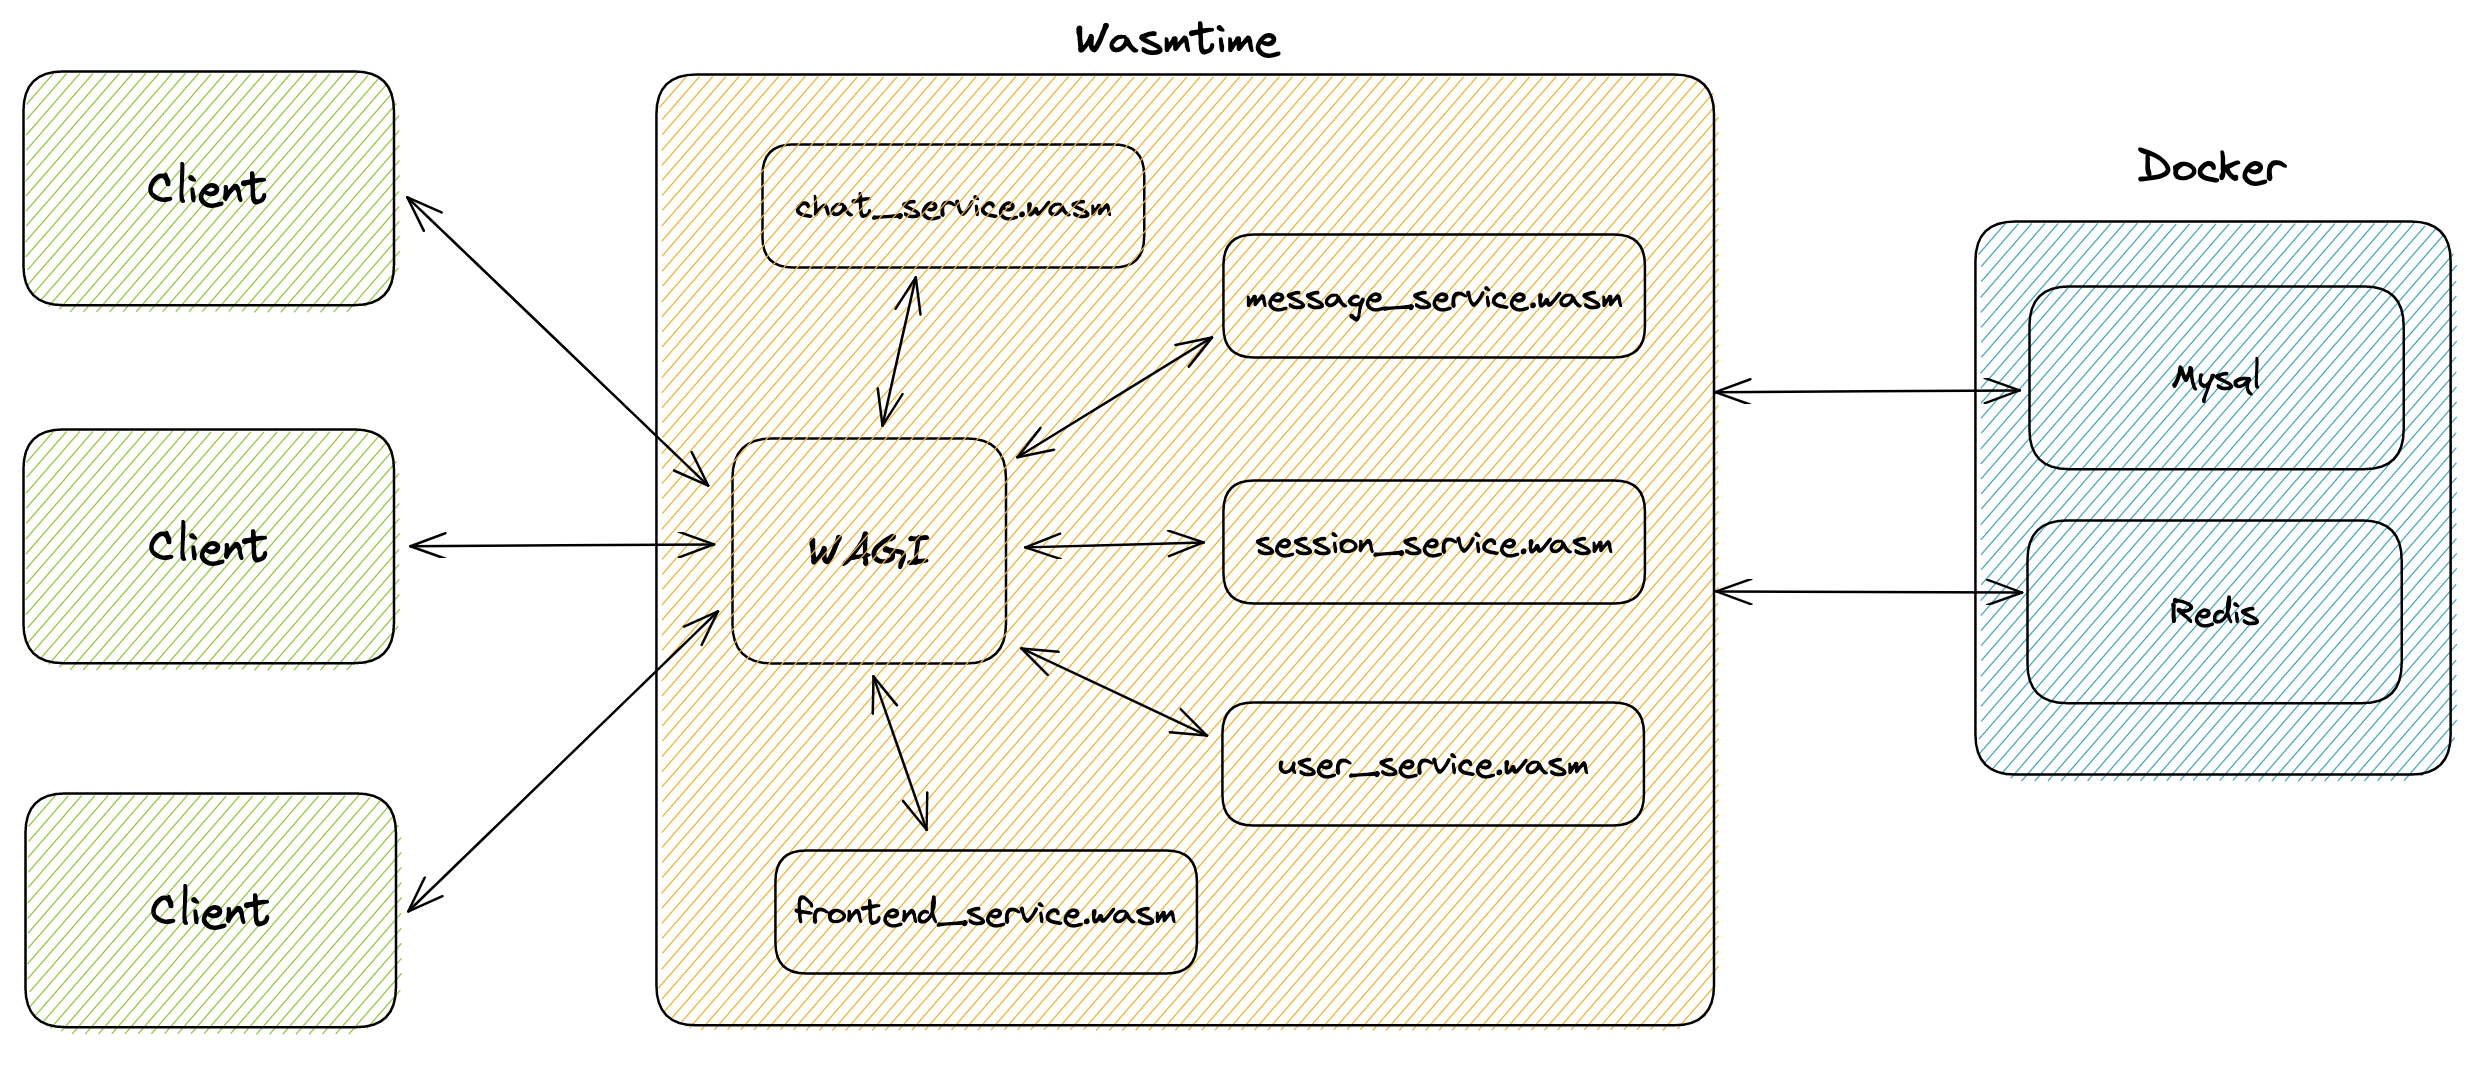
\includegraphics[width=15cm]{./chapters/3.poc/images/0.poc-architecture.png}
    \label{fig:0.poc-architecture}
    \caption{Architettura dell'applicazione}
\end{figure}

\subsection{La configurazione}
La configurazione dell'applicazione avviene modificando il file spin.toml, qui sono presenti varie direttive come la
configurazione delle variabili d'ambiente, del database, di redis e del webserver sottostante. Inoltre qui si
configurano i microservizi presenti nell'applicazione impostando il loro path nella gerarchia delle cartelle, il comando
per eseguire il build e l'url corrispondente ad ognuno di essi. È interessante notare che questo step di mapping tra
url-microservizio-path è necessario poiché il runtime non potrebbe accedere ai vari moduli senza avere le capabilities
necessarie.

\begin{figure}[h]
    \centering
    \captionsetup{justification=centering}
    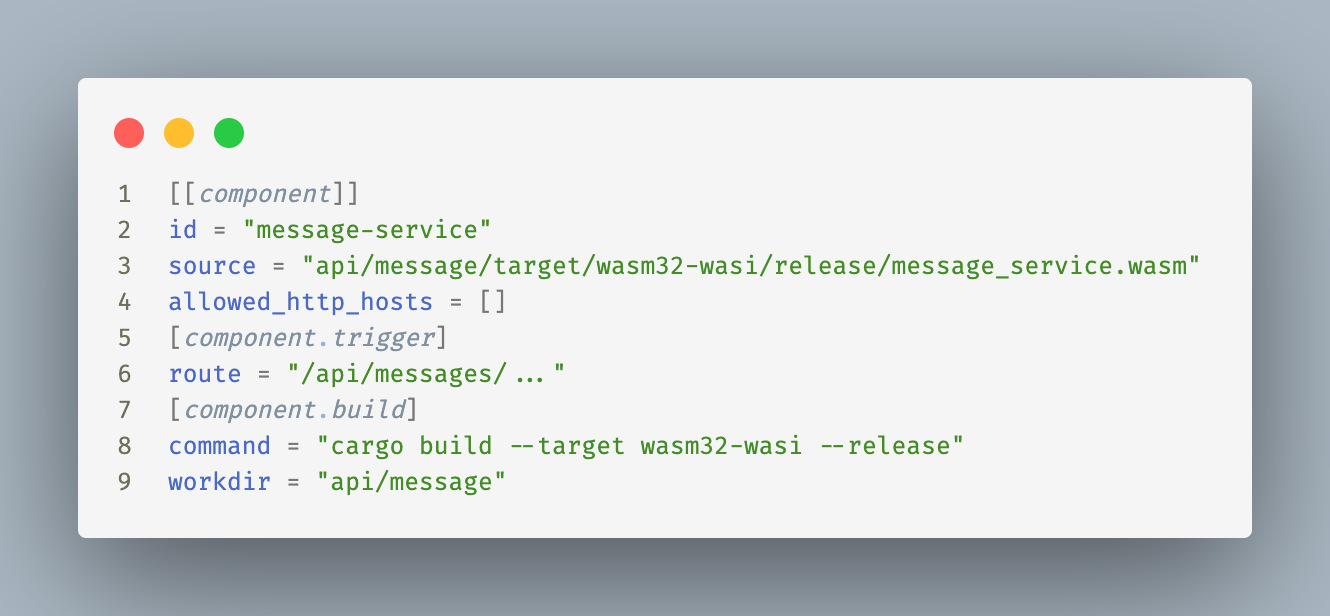
\includegraphics[width=15cm]{./chapters/3.poc/images/1.spintoml.png}
    \label{fig:1.app-configuration}
    \caption{Configurazione di un microservizio}
\end{figure}

Si noti la flag --release nel comando 'cargo build', questa è una direttiva per il compilatore Rust che gli indica di
ottimizzare il codice durante la compilazione.

\subsection{Interazione}
Parliamo ora di come avviene l'interazione tra le componenti dell'applicazione.

L'applicazione viene avviata tramite il comando spin build --up che esegue il build delle componenti definite nel file
di configurazione spin.toml e avvia il web server WAGI in ascolto sulla porta 3000. All'arrivo di una richiesta WAGI,
carica il modulo corrispondente nella sandbox all'url richiesto, se lo trova, e lo avvia con i parametri necessari.
Questo step è trasparente allo sviluppatore in quanto la gestione del web server sottostante è gestita automaticamente.

\begin{figure}[h]
    \centering
    \captionsetup{justification=centering}
    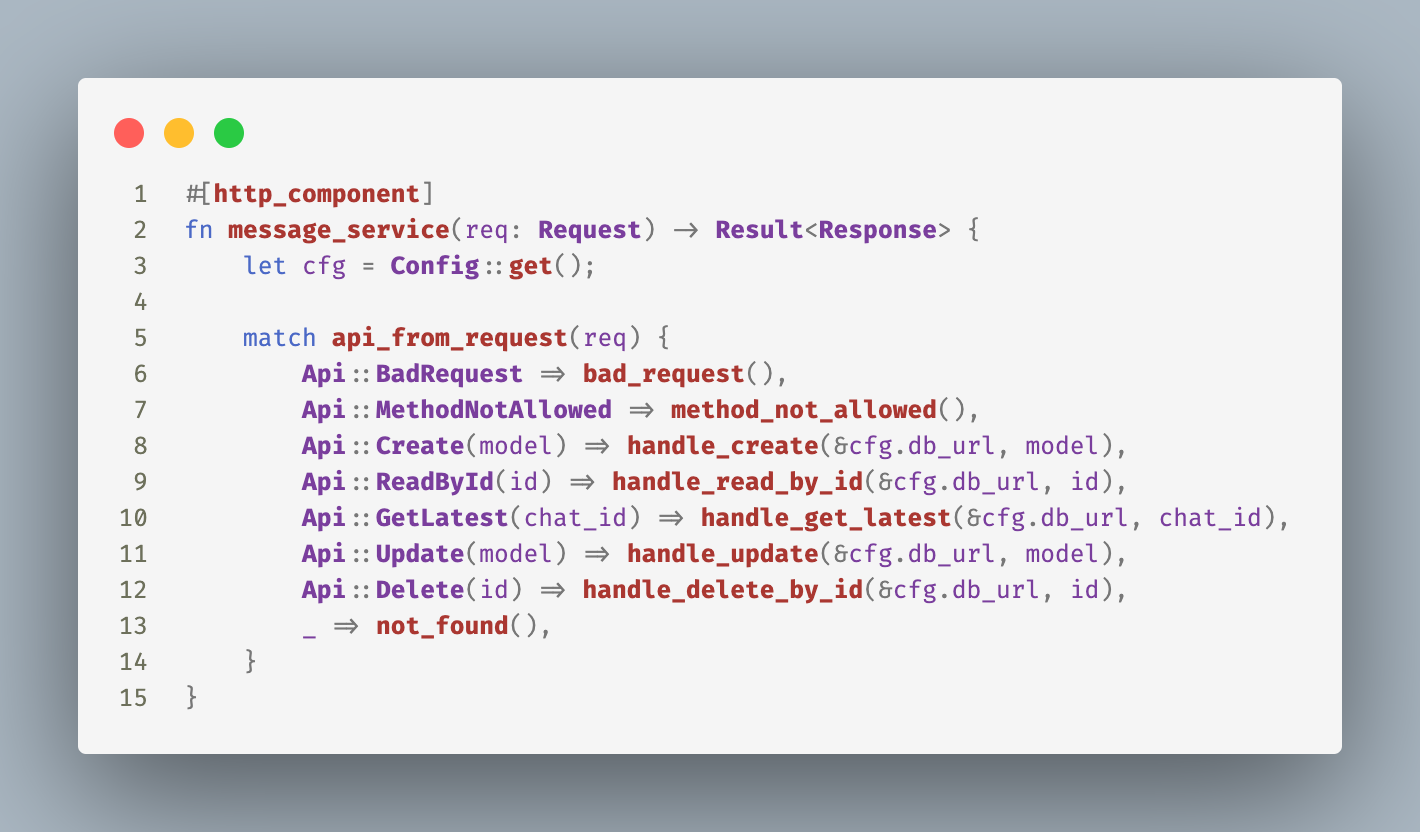
\includegraphics[width=15cm]{./chapters/3.poc/images/2.microservice_entrypoint.png}
    \label{fig:2.microservice_entrypoint}
    \caption{Entry point delle operazioni CRUD al microservizio dei messaggi}
\end{figure}

Il modulo specifica l'entry point attraverso la direttiva \#[http\_component], esegue il parsing della richiesta e ne
elabora la risposta.

La prima interazione tra client e server è necessaria per generare il token di sessione che identifica il cliente che
verrà usato per tutte le richieste successive. Il token viene generato dal session\_service e viene salvato sul
database. Una volta ottenuto, il client può effettuare le richieste all'applicazione.

% Un utente può essenzialmente fare due cose: interagire con le chat e scrivere messaggi. Ogni 

\subsubsection{Una nota sulla sincronizzazione realtime}
La sincronizzazione dei dati in tempo reale tra client e server è effettuata tramite un'interazione a polling. Il motivo
di questa scelta è dato dal fatto che al momento della scrittura del documento WASI non supporta la gestione delle
WebSocket.

\section{Un confronto}
Confrontiamo il microservizio che si occupa della gestione dei messaggi con l'analogo scritto con NodeJS e Express per
vedere le principali differenze. Il codice sorgente è disponibile su
GitHub\footnote{\url{https://github.com/ilcors-dev/bachelor-thesis/tree/main/poc/nodejs-alternative}}.

Intanto si deve notare come il microservizio scritto in NodeJS debba esporre un web server per poter essere raggiunto
dall'esterno mentre il microservizio in Wasm è esposto direttamente da WAGI.

In secondo luogo c'è da notare la gestione di Rust, che risulta sicuramente più complessa, ed è dovuta dal fatto che il
linguaggio è più esigente e richiede un approccio più metodico, mentre l'implementazione in NodeJS è più semplice e
veloce da scrivere ma più prona agli errori runtime.

\subsection{Benchmark}
Andiamo ad analizzare le prestazioni dei due microservizi usando uno strumento chiamato
JMeter\footnote{\url{https://jmeter.apache.org/}}. Il benchmark è stato effettuato su un computer con le seguenti
caratteristiche: CPU Apple M1 8 core e 16 GB di RAM. I test mirano ad analizzare le prestazioni del microservizio in
Wasm e del microservizio in NodeJS in termini di tempo di risposta e di numero di richieste al secondo. Sono stati
effettuati vari benchmark secondo carichi diversi, per i servizi di inserimento dei messaggi. Al ripetersi di ogni test
il database è stato svuotato.

\begin{figure}[!htb]
    \minipage{0.48\textwidth}
        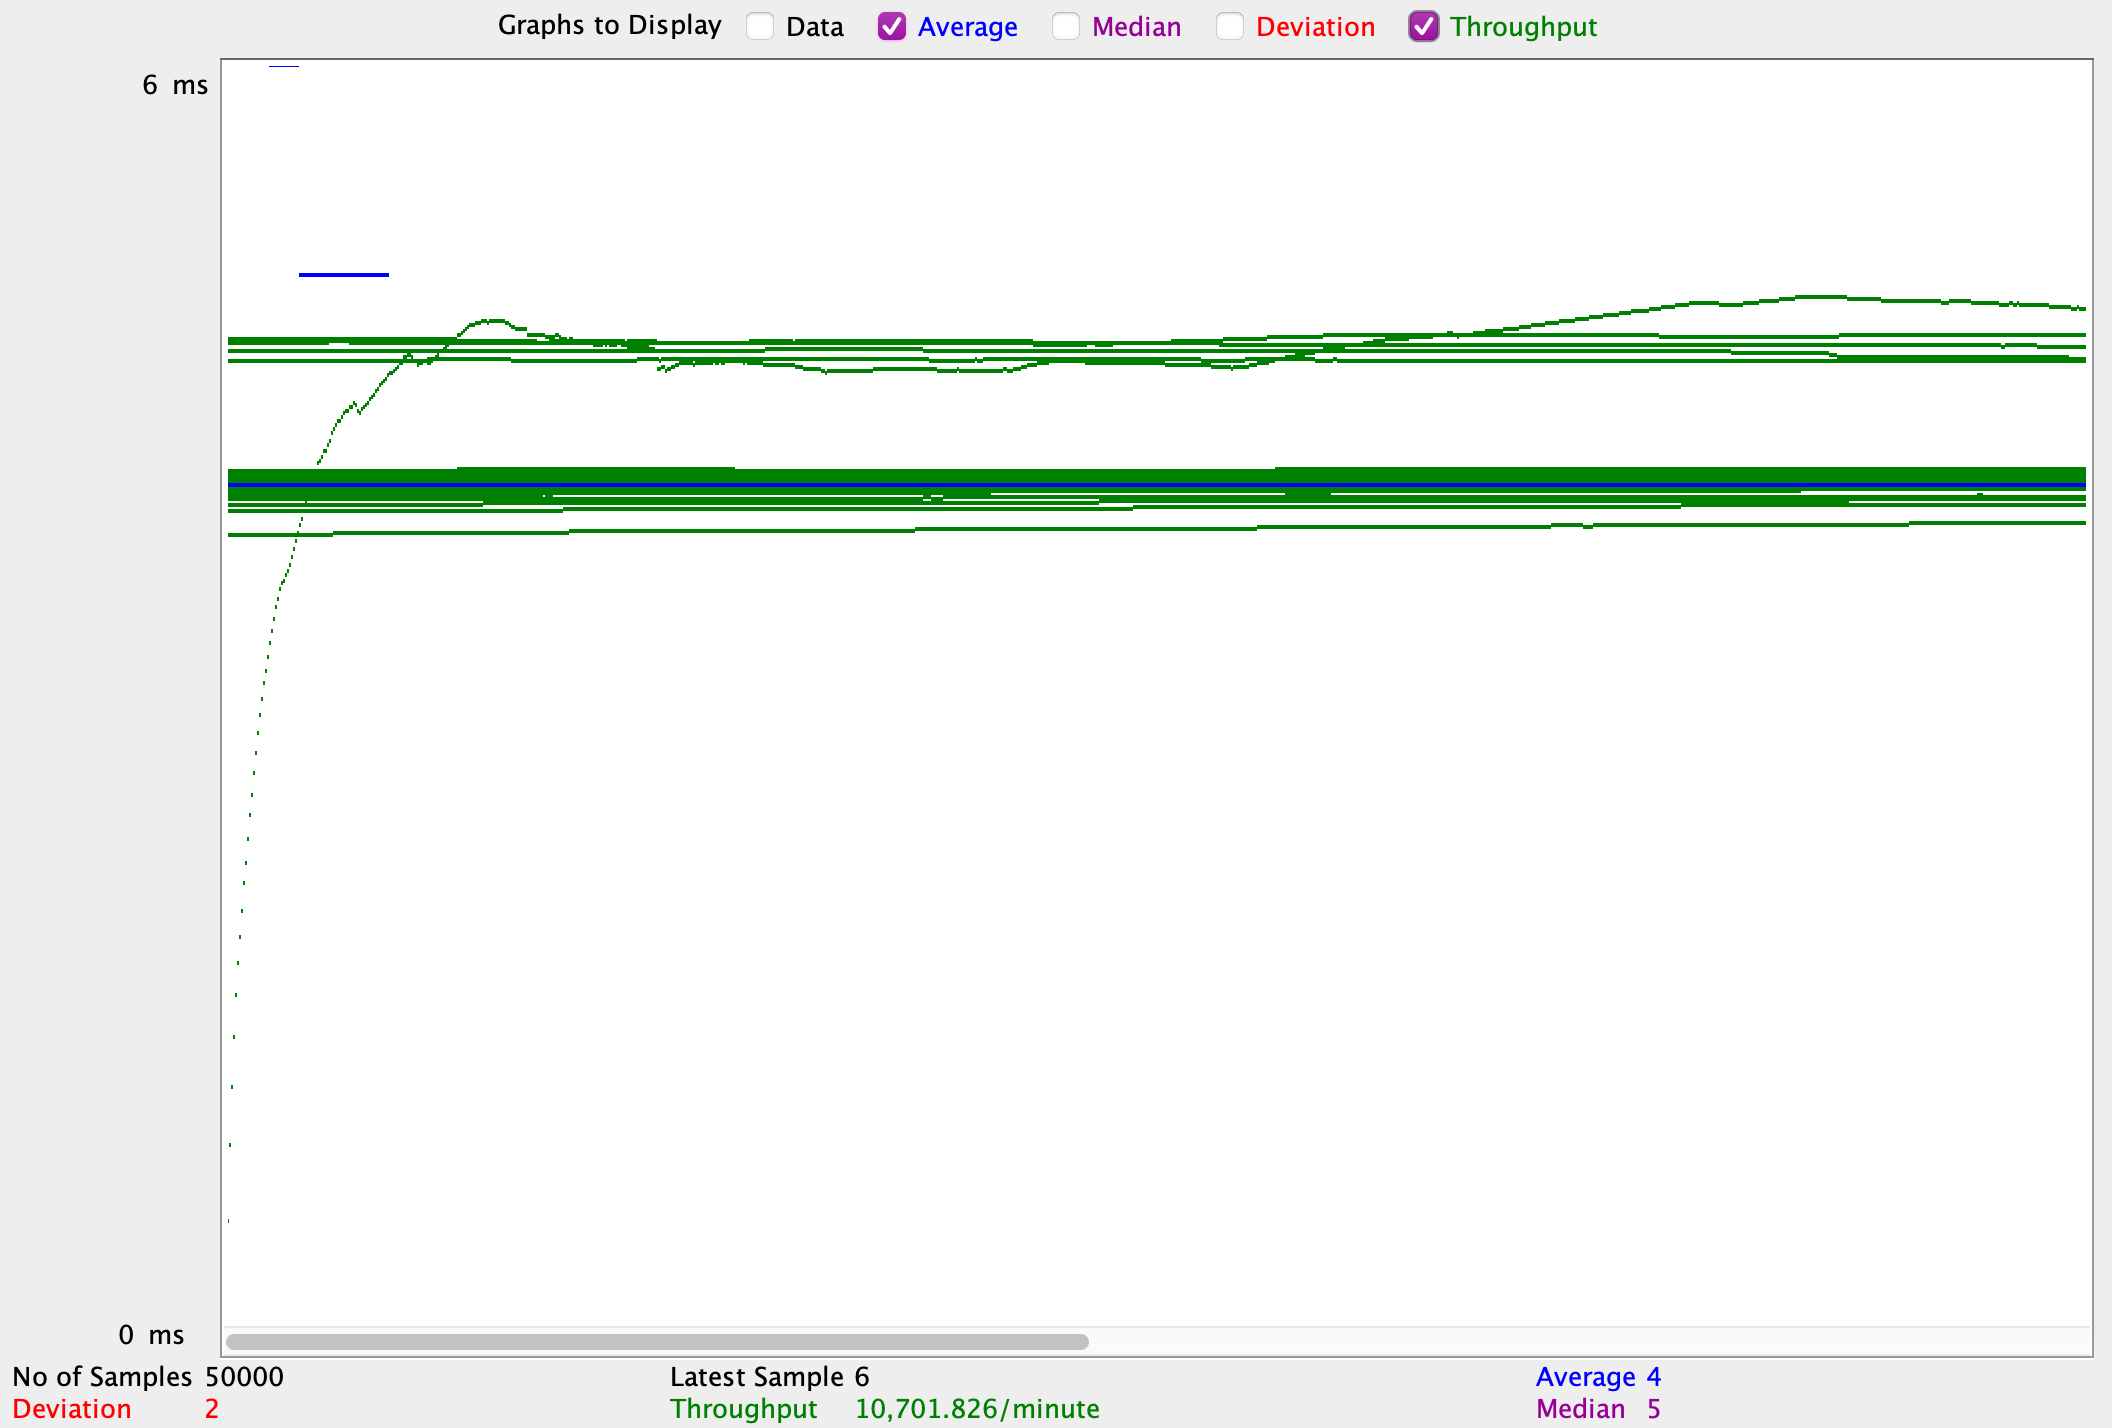
\includegraphics[width=\linewidth]{chapters/3.poc/benchmarks_images/wasi_10000_single_req.png}
        \caption{10000 richieste in sequenza verso Wasm}\label{fig:10000_req_wasi} \endminipage\hfill
    \minipage{0.48\textwidth}
        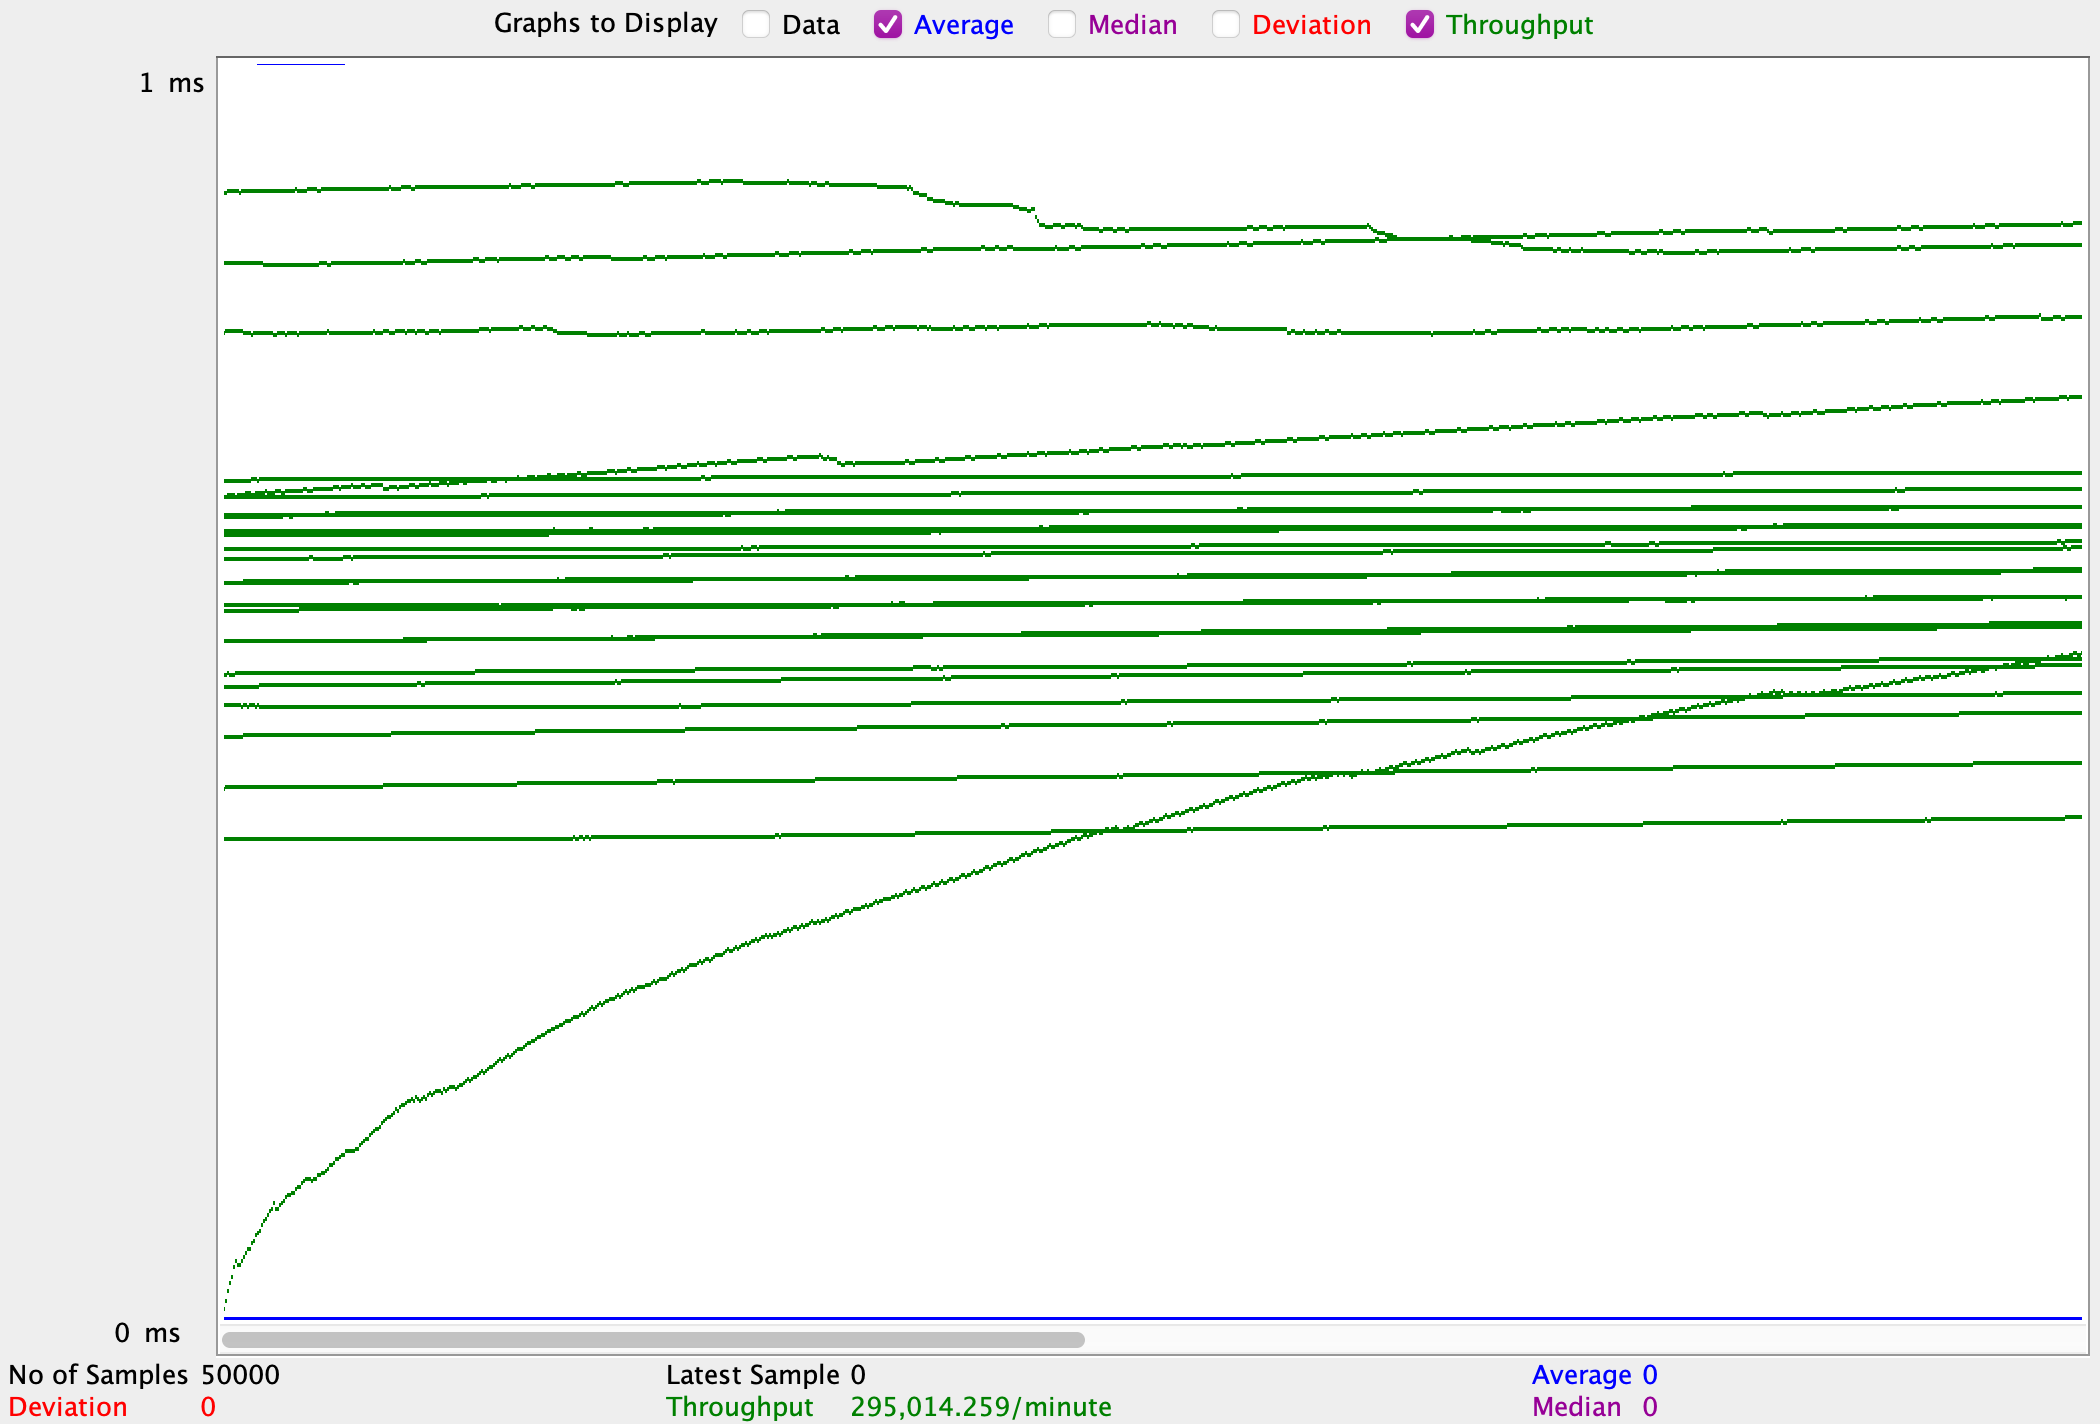
\includegraphics[width=\linewidth]{chapters/3.poc/benchmarks_images/node_10000_single_req.png}
        \caption{10000 richieste in sequenza verso NodeJS}\label{fig:10000_req_node} \endminipage\hfill
\end{figure}

\begin{figure}[!htb]
    \minipage{0.48\textwidth}
        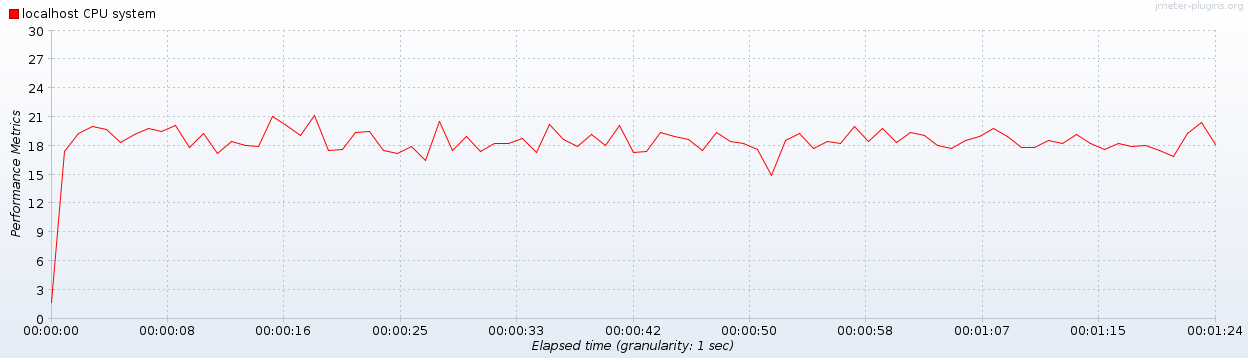
\includegraphics[width=\linewidth]{chapters/3.poc/benchmarks_images/wasi_10000_single_req_cpu.png}
        \caption{Utilizzo CPU per Wasm}\label{fig:10000_req_wasi_cpu} \endminipage\hfill
    \minipage{0.48\textwidth}
        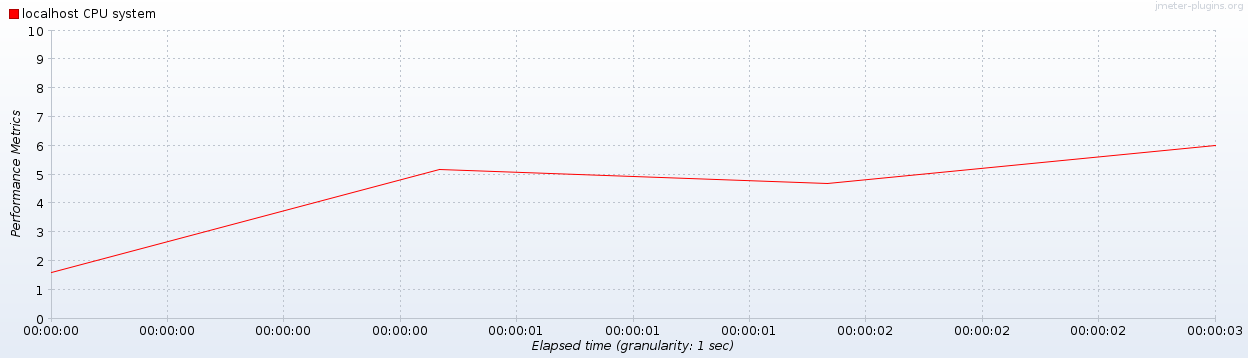
\includegraphics[width=\linewidth]{chapters/3.poc/benchmarks_images/node_10000_single_req_cpu.png}
        \caption{Utilizzo CPU per NodeJS}\label{fig:10000_req_node_cpu} \endminipage\hfill
\end{figure}

Il primo test effettuato mira a valutare le prestazioni dei due servizi sotto un carico di 10000 richieste effettuate in
modo sequenziale. Il test è stato ripetuto 5 volte, per un totale di 50000 richieste. Si può notare come Wasm non riesca
a soddisfare al carico di richieste come NodeJS. Nel primo caso i tempi di risposta risultano essere tra i 4ms e i 6ms
mentre nel secondo sono tutti sotto al millisecondo. Vediamo ora come si comportano i due nel gestire richieste in
parallelo ovvero simulando l'utilizzo del servizio da parte di più utenti nello stesso momento.

\begin{figure}[H]
    \minipage{0.48\textwidth}
        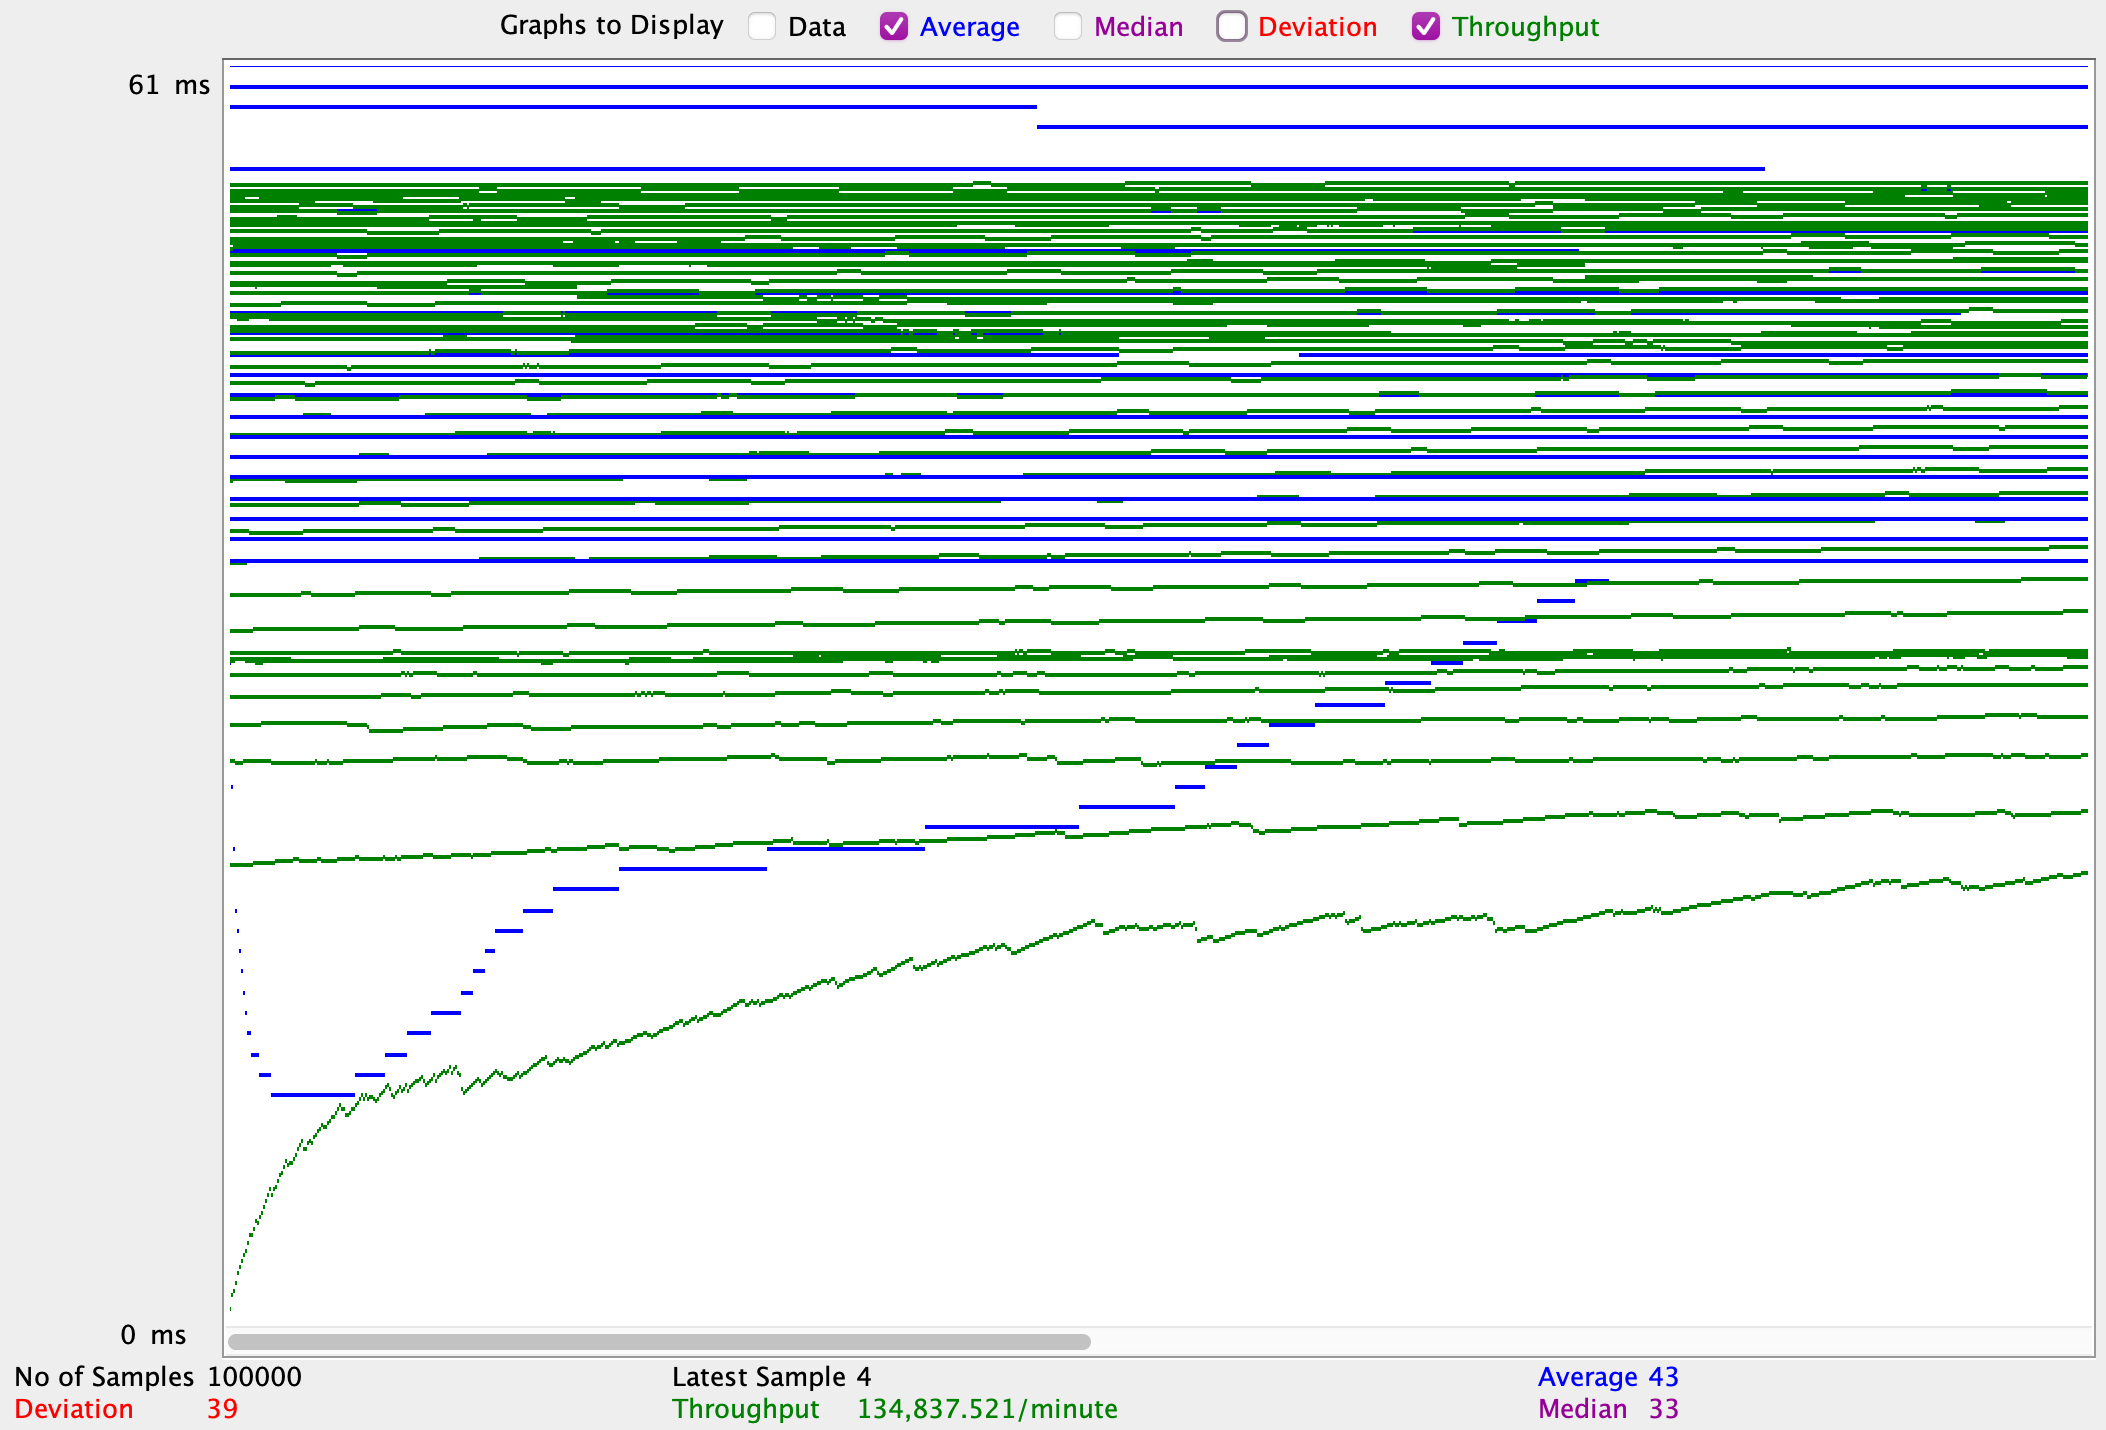
\includegraphics[width=\linewidth]{chapters/3.poc/benchmarks_images/wasi_100_thread_1000_req.png}
        \caption{100 utenti e 1000 richieste in simultanea verso Wasm}\label{fig:100_thread_1000_req_wasi}
    \endminipage\hfill
    \minipage{0.48\textwidth}
        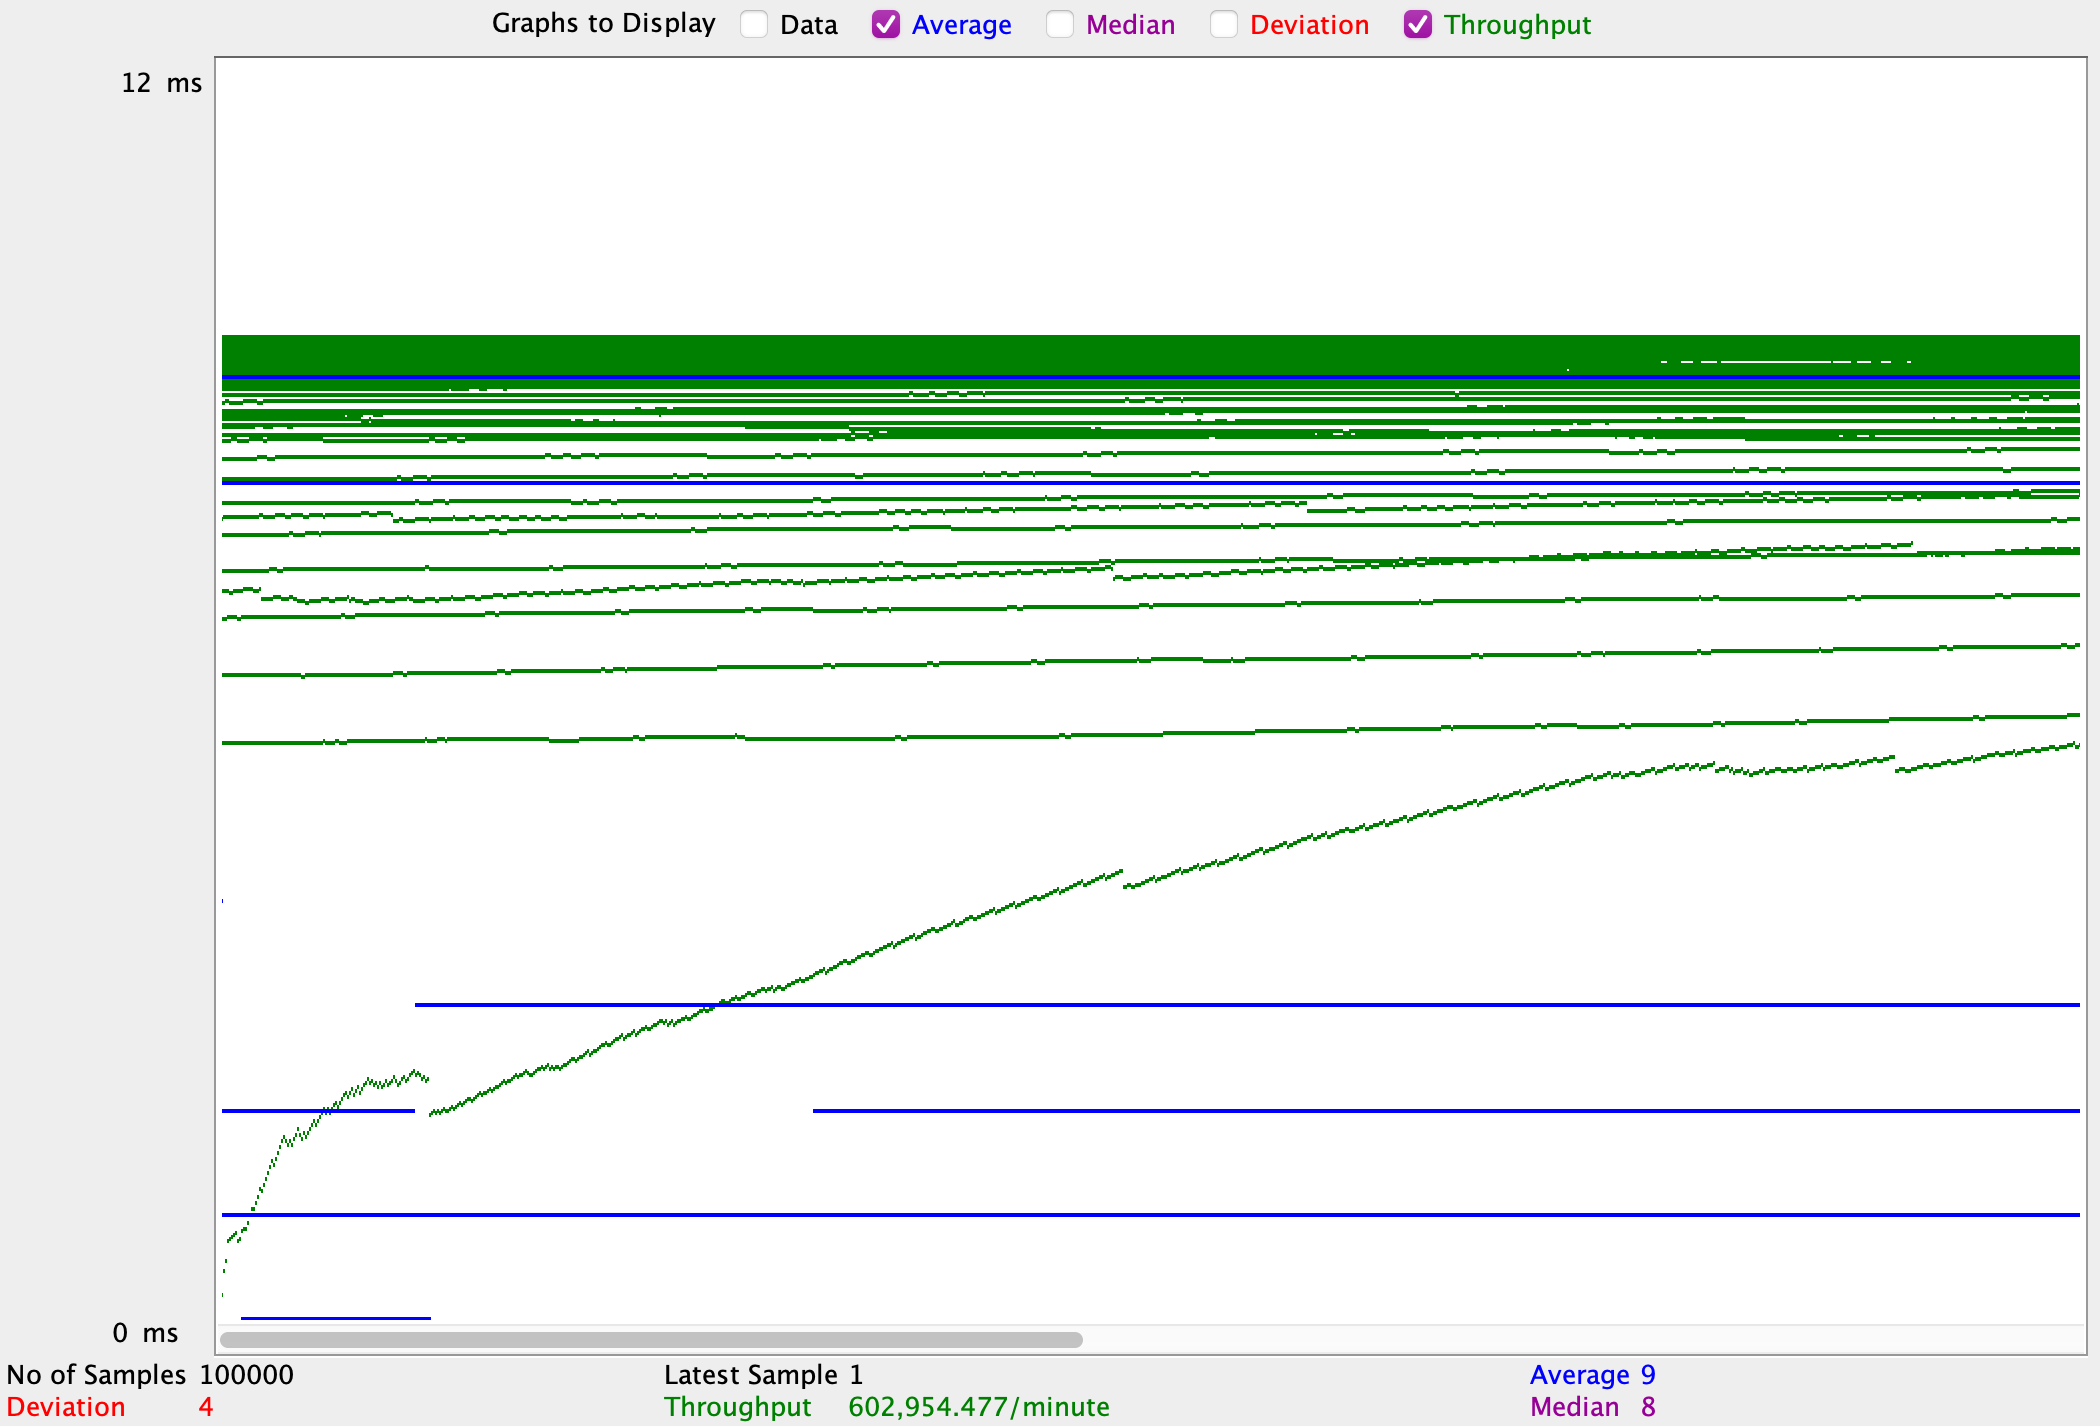
\includegraphics[width=\linewidth]{chapters/3.poc/benchmarks_images/node_100_thread_1000_req.png}
        \caption{100 utenti e 1000 richieste in simultanea verso NodeJS}\label{fig:100_thread_1000_req_node}
    \endminipage\hfill
\end{figure}

\begin{figure}[H]
    \minipage{0.48\textwidth}
        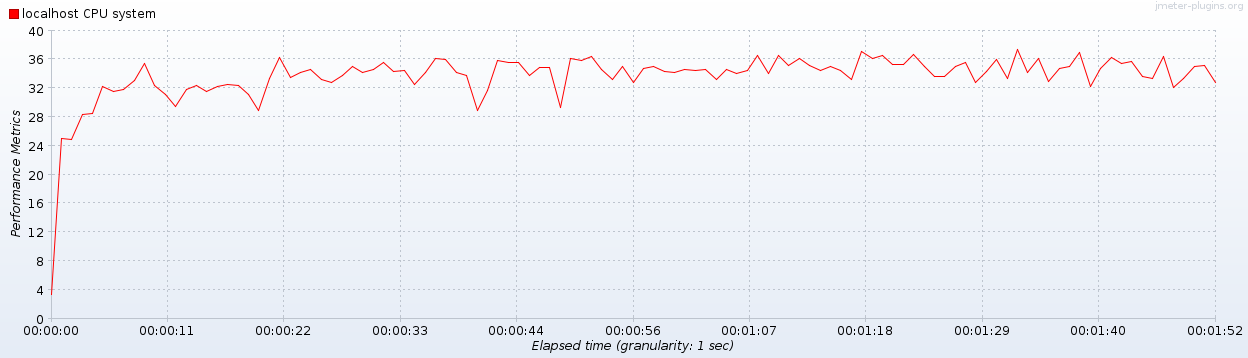
\includegraphics[width=\linewidth]{chapters/3.poc/benchmarks_images/wasi_100_thread_1000_req_cpu.png}
        \caption{Utilizzo CPU per Wasm}\label{fig:100_thread_1000_req_wasi_cpu}
    \endminipage\hfill
    \minipage{0.48\textwidth}
        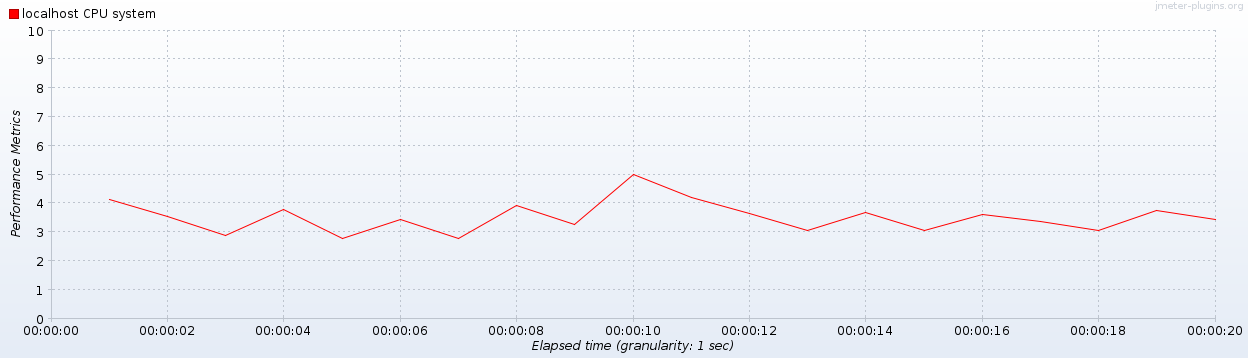
\includegraphics[width=\linewidth]{chapters/3.poc/benchmarks_images/node_100_thread_1000_req_cpu.png}
        \caption{Utilizzo CPU per NodeJS}\label{fig:100_thread_1000_req_node_cpu}
    \endminipage\hfill
\end{figure}

Anche in questo caso Wasm non regge il confronto con NodeJS. Il primo ha tempi di risposta che arrivano fino ai 60ms
mentre il secondo non supera i 12ms.

\subsection{Il deployment}
Valutiamo ora invece la gestione del deployment delle due soluzioni. In entrambi i casi si è scelto di creare due
immagini dell'applicazione che seguano lo standard OCI. OCI è un formato comune per le immagini container che definisce
uno standard per la creazione, la distribuzione e l'esecuzione di essi. Per creare l'immagine dell'applicazione NodeJS è
stato utilizzato il seguente Dockerfile: 

\begin{figure}[!htb]
    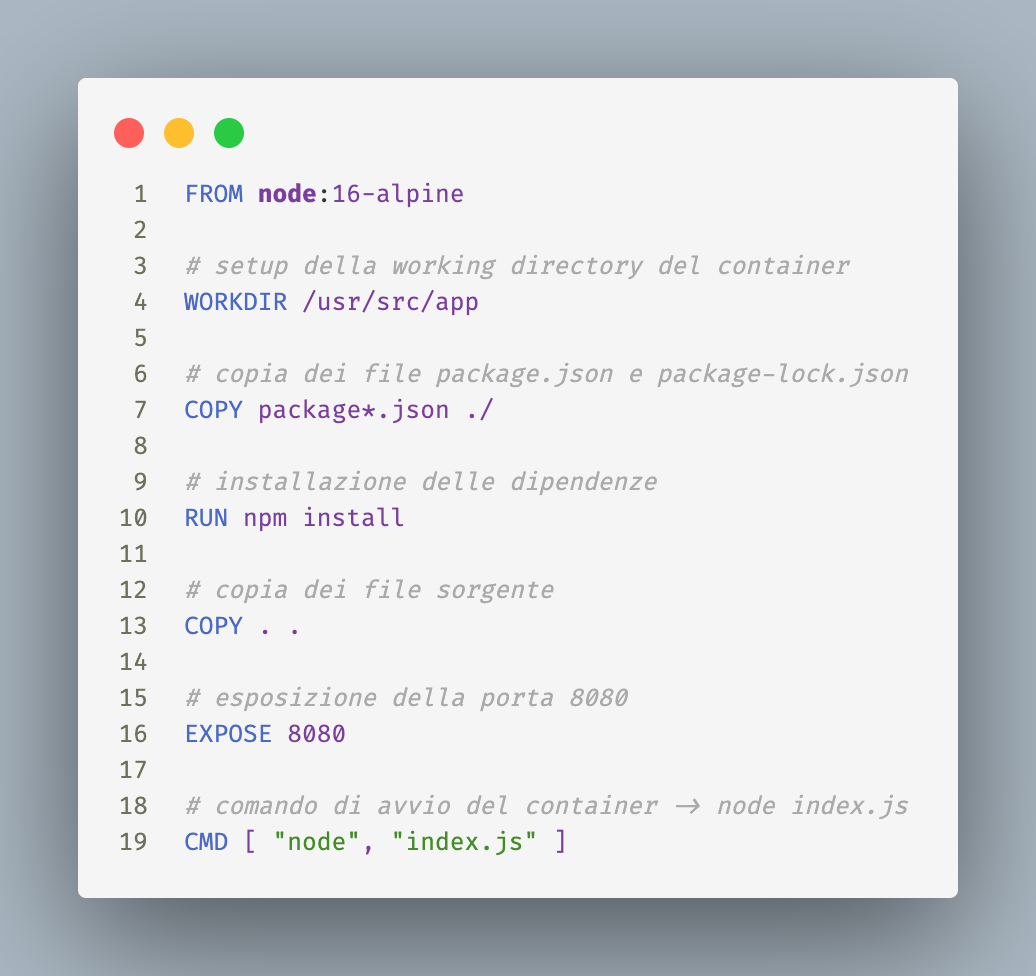
\includegraphics[width=\linewidth]{chapters/3.poc/images/3.nodejs-dockerfile.png}
    \caption{Creazione immagine Docker per l'applicazione NodeJS}\label{fig:nodejs-dockerfile}
\end{figure}
    
Il Dockerfile ci permette di creare l'immagine dell'applicazione tramite il comando.
\begin{verbatim}
docker buildx build . -t ghcr.io/ilcors-dev/chat-nodejs:latest
\end{verbatim}

e di pubblicarla su GitHub Container Registry (GHCR), un gestore di immagini container, tramite

\begin{verbatim}
docker push ghcr.io/ilcors-dev/chat-nodejs:latest
\end{verbatim}

Per l'immagine dell'applicazione WASI invece è stato utilizzato il tool integrato nel
\hyperref[sec:spin-framework]{Framework Spin} che ci permette, tramite

\begin{verbatim}
    spin registry push ghcr.io/ilcors-dev/wasi-chat-poc:latest
\end{verbatim}

di creare l'immagine e di pubblicarla su GHCR. Entrambe le immagini sono reperibili al seguente link:
\url{https://github.com/ilcors-dev?tab=packages}

Possiamo analizzare le differenze tra le due soluzioni in termini di dimensioni su disco. Si può notare, attraverso
l'image manifest reperibile direttamente dall'interfaccia utente del sito, come quella di NodeJS sia estremamente più
pesante di quella di Wasm nonostante includa le stesse funzionalità. La prima occupa uno spazio di
65MB\footnote{\url{https://github.com/users/ilcors-dev/packages/container/chat-nodejs/76069897?tag=latest}} circa,
mentre la seconda appena
2,4MB\footnote{\url{https://github.com/users/ilcors-dev/packages/container/wasi-chat-poc/76056566?tag=latest}}

Questo è dovuto al fatto che l'applicazione Wasm è già pronta per essere eseguita in un runtime Wasm e non necessita di
altre dipendenze, mentre l'applicazione NodeJS deve, oltre ad includere tutte le dipendenze necessarie, essere eseguita
su NodeJS all'interno di una versione leggera di Linux, chiamata Alpine Linux.

Avendo entrambe le immagini disponibili su GHCR è possibile effettuare il deployment delle due applicazioni in locale.

Per l'applicazione NodeJS è necessario configurare sia il container per l'applicazione che il container per la
persistenza dei dati tramite il file docker-compose.yml:

\begin{figure}[!htb]
    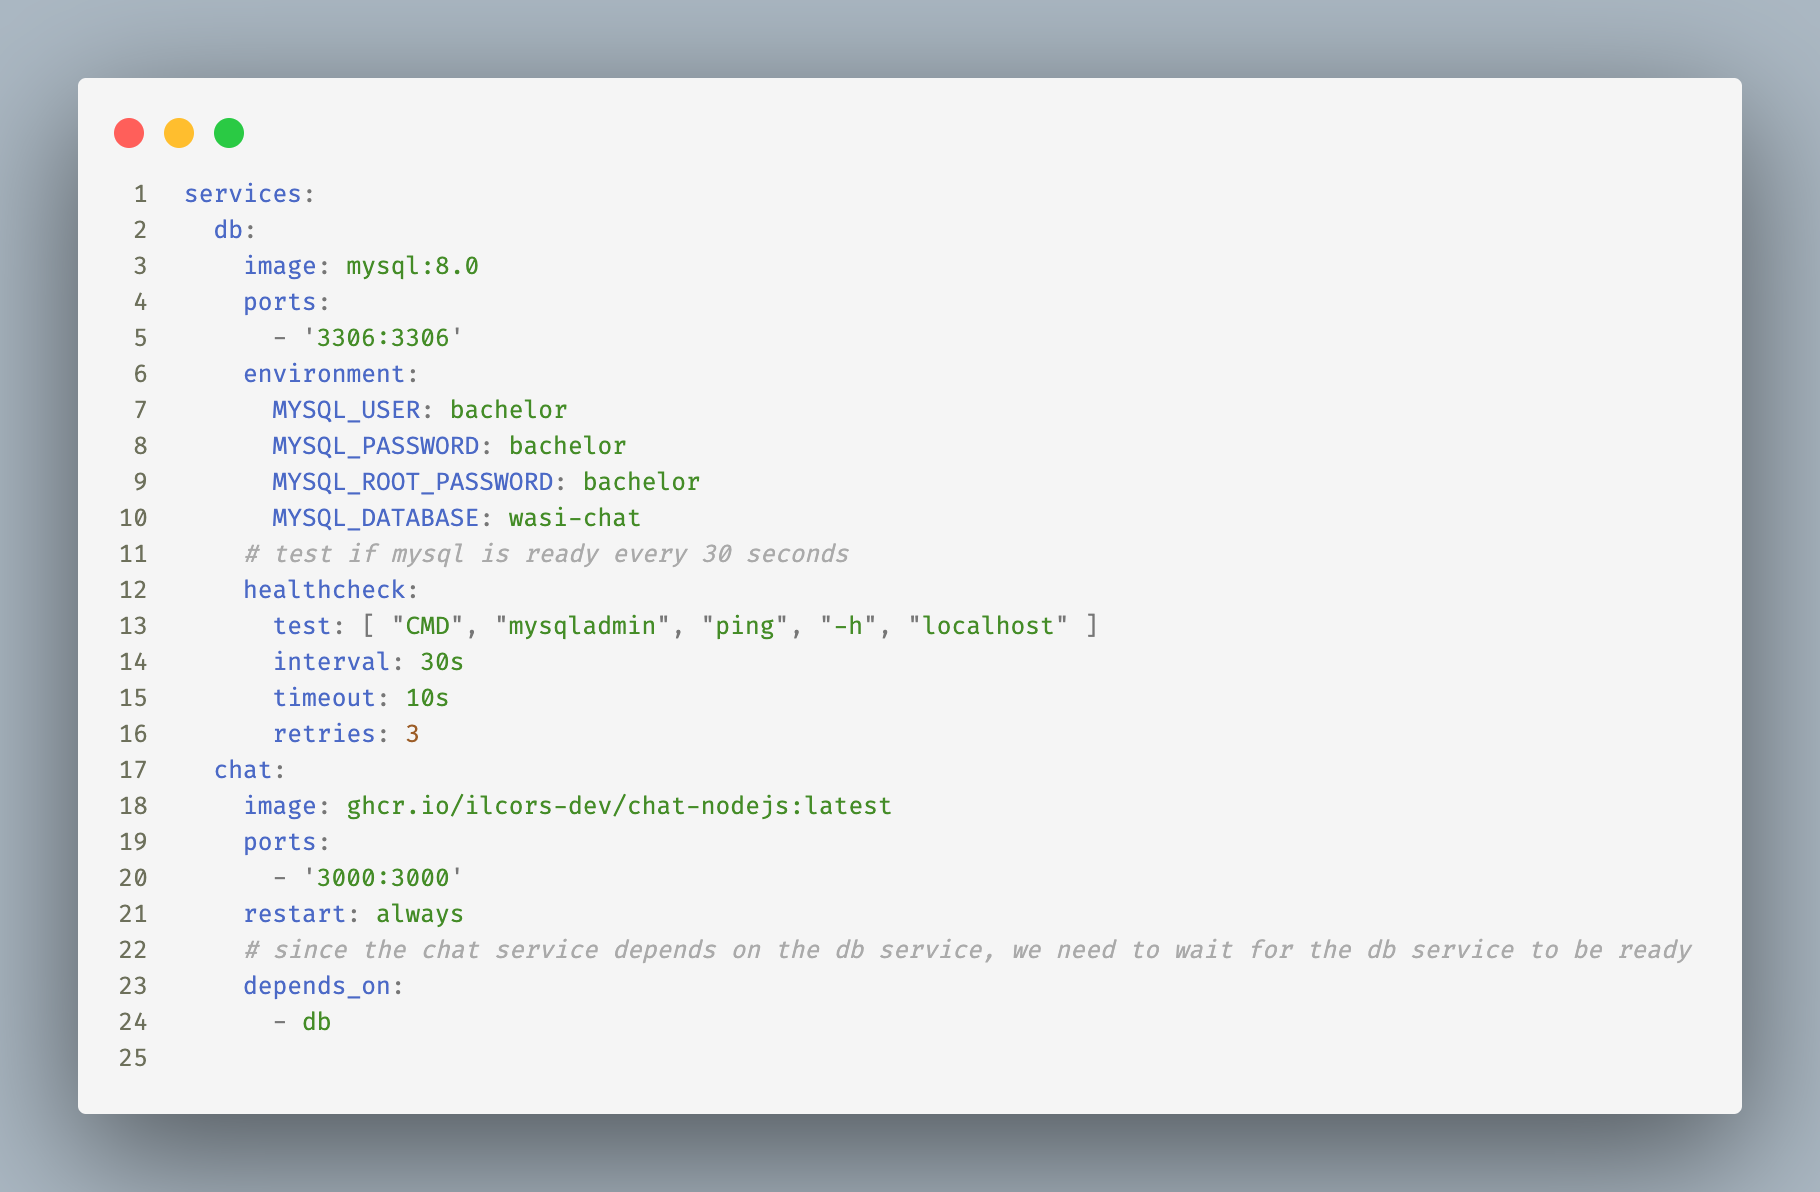
\includegraphics[width=\linewidth]{chapters/3.poc/images/5.docker-compose-nodejs.png}
    \caption{Docker compose per l'applicazione NodeJS}\label{fig:nodejs-dockercompose}
\end{figure}

e per eseguirla è sufficiente il comando

\begin{verbatim}
docker-compose up
\end{verbatim}

Anche per l'applicazione Wasm è necessario usare Docker Compose, ma solo per avviare il container per la persistenza.
Non se ne riporta l'esempio in quanto è identico a quello precedentemente a meno della configurazione dell'applicazione
NodeJS. Per eseguire l'applicazione Wasm è sufficiente il comando
\begin{verbatim}
    spin up -f ghcr.io/ilcors-dev/wasi-chat-poc:latest
\end{verbatim}

che si occupa di eseguire un pull dell'immagine e di eseguirla in locale.

\section{Vantaggi e Svantaggi}
Nella soluzione proposta per l'applicazione, l'utilizzo di Wasm ha dimostrato di avere sia vantaggi che svantaggi. Da un
lato, ha permesso una maggiore facilità di deployment dell'applicazione grazie alla sua portabilità e alla possibilità
di eseguire il codice su diverse piattaforme. D'altra parte, tuttavia, ha avuto un impatto negativo sulle prestazioni
dell'applicazione.

Questa nota negativa è dovuta principalmente allo stato ancora acerbo di WASI, il quale non è ancora altrettanto maturo
come quello della controparte NodeJS preso in esame. Tuttavia, con il passare del tempo e l'evoluzione della tecnologia,
è probabile che WASI diventi sempre più efficiente e performante.

Inoltre, è importante notare che ogni microservizio dell'applicazione NodeJS richiede la sua modalità di deployment, che
può essere un'operazione complicata e richiedere molto tempo. Invece, l'applicazione Wasm offre un vantaggio
significativo in questo senso, poiché Wasmtime e WAGI si occupano dell'esposizione del server HTTP e includono già tutti
i microservizi necessari per l'esecuzione dell'applicazione.

Infine, è importante evidenziare come l'utilizzo combinato di Docker e WASI rappresenti una soluzione ideale per lo
sviluppo di applicazioni complesse. In particolare, Docker offre una piattaforma completa per la costruzione dei
container e l'esecuzione delle tecnologie complementari necessarie all'applicazione, rappresentando la spina dorsale del
sistema. Mentre, WASI offre la portabilità e la sicurezza del codice Wasm, consentendo di eseguire moduli altamente
ridotti in una sandbox isolata e garantendo la compatibilità dell'applicazione su diverse piattaforme. Insieme, queste
tecnologie consentono di semplificare il processo di deployment dell'applicazione, garantire la scalabilità del sistema
e ridurre i tempi di sviluppo.